\documentclass[onecolumn, draftclsnofoot,10pt, compsoc]{IEEEtran}
\usepackage{graphicx}
\usepackage{url}
\usepackage{setspace}
\usepackage{geometry}
\usepackage{tabularx}
\geometry{textheight=9.5in, textwidth=7in}

\def \CapstoneTeamName{		    Comedy Robot Team}
\def \CapstoneTeamNumber{		43}
\def \GroupMemberOne{			Timothy Bui}
\def \GroupMemberTwo{			Yuhang (Tony) Chen}
\def \GroupMemberThree{			Brian Ozarowicz}
\def \GroupMemberFour{			Trevor Webster}
\def \CapstoneProjectName{		Building More Self-Aware\linebreak Everyday Robots}
\def \CapstoneSponsorCompany{	SHARE Lab}
\def \CapstoneSponsorPerson{	Dr. Naomi Fitter}

% Uncomment the appropriate line below so that the document type works
\def \DocType{	%Problem Statement
				%Requirements Document
				%Technology Review
				Design Document
				%Progress Report
				}
			
\newcommand{\NameSigPair}[1]{\par
\makebox[2.75in][r]{#1} \hfil 	\makebox[3.25in]{\makebox[2.25in]{\hrulefill} \hfill		\makebox[.75in]{\hrulefill}}
\par\vspace{-12pt} \textit{\tiny\noindent
\makebox[2.75in]{} \hfil		\makebox[3.25in]{\makebox[2.25in][r]{Signature} \hfill	\makebox[.75in][r]{Date}}}}
% If the document is not to be signed, uncomment the RENEWcommand below
\renewcommand{\NameSigPair}[1]{#1}

%%%%%%%%%%%%%%%%%%%%%%%%%%%%%%%%%%%%%%%
\begin{document}
\begin{titlepage}
    \pagenumbering{gobble}
    \begin{singlespace}
    	
\includegraphics[height=4cm]{coe_v_spot1}
        \hfill 
        % If you have a logo, use this includegraphics command to put it on the coversheet.
        %\includegraphics[height=4cm]{CompanyLogo}   
        \par\vspace{.2in}
        \centering
        \scshape{
            \huge CS Capstone \DocType \par
            %{\large\today}\par
            {\large Fall 2019}\par
            \vspace{.5in}
            \textbf{\Huge\CapstoneProjectName}\par
            \vfill
            {\large Prepared for}\par
            %\Huge \CapstoneSponsorCompany\par
            %\vspace{5pt}
            {\Large\NameSigPair{\CapstoneSponsorPerson}\par}
            {\large Prepared by }\par
            Group\CapstoneTeamNumber\par
            % comment out the line below this one if you do not wish to name your team
            \CapstoneTeamName\par 
            \vspace{5pt}
            {\Large
                \NameSigPair{\GroupMemberOne}\par
                \NameSigPair{\GroupMemberTwo}\par
                \NameSigPair{\GroupMemberThree}\par
                \NameSigPair{\GroupMemberFour}\par
            }
            \vspace{20pt}
        }
        \begin{abstract}
        	\noindent The goal of this project is to improve a robot's ability to determine if a joke was a hit or a bomb based on the audience laughter. The tasks involved in achieving this goal are collecting audio data of the audience responses, preprocessing the data by applying noise suppression and normalization, and performing machine learning on the data to train models for automated joke classification. The classification success rate should be at least 85\% when used on a dataset of pre-recorded jokes. Once the learning model operates successfully on the offline dataset it will be moved onboard the robot for real-time usage.
        \end{abstract}
    \end{singlespace}
\end{titlepage}
\newpage
\pagenumbering{arabic}
\tableofcontents
% uncomment this (if applicable). Consider adding a page break.
%\listoffigures
%\listoftables
\clearpage

\section{Glossary}
\vspace{.3cm}
\begin{tabularx}{\linewidth}{l|X}
\textbf{Term} & \textbf{Definition} \\ \hline
Machine Learning & Using patterns in data to automate analytical decision making without needing human input \\ \hline
NAO Robot (pronounced Now) & An autonomous, programmable humanoid robot \\ \hline
Noise Suppression & A method of enhancing audio data by giving the input a higher signal-to-noise ratio \\ \hline
Praat & A software package designed for speech analysis. \\ \hline                                 
Python & An interpreted, general-purpose programming language \\ \hline                                 
SciKit & A Python library for performing software machine learning \\ \hline                              
SSD (solid-state drive) & A storage device with quicker access time than a hard drive with a spinning disk \\ \hline                              
\end{tabularx}
\vspace{.2cm}

\section{Introduction}
\subsection{Goals and Objectives}
This project involves studying robot-human communication by observing interactions in a stand-up comedy setting. This document provides design details of the components that will be used for our work in using machine learning to improve the ability of a robot to analyze audience laughter and will outline how our team plans to accomplish the goals that we were tasked with when taking on this project.\par
\vspace{.3cm}
\noindent Dr. Naomi Fitter wants to be able to improve the accuracy of detecting human laughter in response to jokes told by a robot, as well as adding the ability to detect human laughter while a joke is being told by the robot. This will require work in the fields of real-time audio manipulation as well as audio analysis and machine learning. Work done on this project can also contribute to the greater field of human-computer interaction. Progress on this project can lead to enhanced accuracy in the ability of robots to analyze human behavior and responses. The primary functions of the tool our team is creating will be to gather, analyze, and classify audio data from an audience in real-time.\par
\subsection{Statement of Scope}
The scope of the project being developed by our team will be to create a tool to classify jokes as a hit, a bomb, or somewhere in between based on how the audience reacted. Modularity will aid with future efforts to improve and expand the utility of the tool. The capstone team will primarily be utilizing Python and SciKit to develop the tools. The user of this tool will primarily be Dr. Fitter and any other individuals aiding her with the robot comedy performance. The users can interact with our tool via command-line interface. This tool aims to be a natural extension of the pre-existing program already in use by the robot team. The output of this tool will be dependent on the audio input that we receive. This audio can change depending on various factors such as microphone quality and venue. For this project we will be taking audio input using the robot's onboard microphones. If necessary we could also use the cameras onboard the NAO robot; this, however, is not our primary goal, but an additional avenue that our team can pursue should the need arise.

\section{Constraints}
There are several factors our group must take into account regarding the performance of the NAO V6 Robot. First, all of the programs and scripts used for data processing and normalization must have a small enough file size to fit within the 128GB SSD storage capacity of the NAO V6 Robot. There must also be enough room for the robot to store its database of jokes and its operating system. This limits the number and size of the programs that can be used for data preprocessing.\par
\vspace{.3cm}
\noindent Second, the jokes must be able to be preprocessed, normalized, and classified in real time by the NAO V6 Robot. The NAO V6 Robot has a SSD which will allow for rapid file reading and writing and uses an Intel Atom 4 core 1.95 GHz Processor. Furthermore, the classifiers themselves do not need to be created on the robot. The data collection, preprocessing, normalization, and classification however does need to be performed in real time. Only one mp3 file needs to be classified at a time during performances.\par
\vspace{.3cm}
\noindent Third, while our group will be working with the NAO V6 robot, a significant portion of the audio data our group has to work with was obtained using a NAO V5 robot. The NAO V6 includes significantly better microphones which creates cleaner audio files. As a result, our group will need to take care not to overfit the machine learning algorithms to work well on the older audio files.

\section{Methods}
\subsection{Overview}
Our team will work primarily within the existing structure of the project. Raw audio data from prior performances by the robot is stored in a database as mp3 files. Our team will process the data by creating a program that imports the mp3 files, cleans the audio and converts it into measurable data, then normalizes that data. A portion of the data will be set aside for testing, while the rest of the data will be used to train a classifier. Once the classifier has been created, the group will test the classifier using the data that had previously been set aside. Our group will repeat this task using different data processing and classification methods and recording the results of our testing to determine which approaches generate the best results consistently. The goal is for the automated system to achieve an 85\% accurate classification rate or better, to match the performance observed when humans are doing the joke classification.
\subsection{Data Collection}
The data is recorded via the NAO V6 robot's onboard microphones during live performances and stored as mp3 files on the robot's SSD. After performances the data will be backed up on a secure server and a second copy will be made to use as training data for the classifier. The original data stored on the robot will be deleted in order to save space on the robot's SSD for future performances. A large portion of the data has already been hand sorted as either a hit, a bomb, or somewhere inbetween.
\subsection{Data Processing}
The data preprocessing can be split into three forms: noise suppression, data extraction, and normalization. Noise suppression techniques can improve the audio quality of the mp3 file and therefore the quality of the data we are able to extract from the file. Different techniques will need to be used based on whether the mp3 file is used to look for post-joke audience reactions or mid-joke audience reactions since mp3 files with mid-joke reactions will also include the sound of the robot's voice. Time will be a major consideration during our testing of the noise suppression algorithms since they must be capable of being run in real time during a live performance.\par
\vspace{.3cm}
\noindent Data extraction will be done using Praat, a lightweight program that can extract data such as intensity, pitch, frequency, and minimum and maximum volume from the mp3 files.\par
\vspace{.3cm}
\noindent The two most standard normalization techniques are min-max scaling and z-scaling. Min-max provides better direct comparisons since the data will always be on the same scale, while z-scaling is more robust at handling outliers. Which of the two will perform best for our use will depend largely on how successful the noise suppression is and the type of data being analyzed, so our team will test each type of normalization for each iteration of the noise suppression to determine what produces the best results.
\subsection{Training Models}
After the audio has been processed from mp3 files into data our group will use a variety of machine learning methods to train classification models for determining whether a joke was a hit, a bomb or somewhere inbetween. A portion of the data must be set aside for later testing of the results prior to training the algorithm. In order to speed up our process, machine learning algorithms provided via SciKit can be used when appropriate. Each training algorithm will be tried with different setting parameters and on different data processing techniques. Once the classifier has been created it can then be extracted and used to classify data.
\subsection{Validation Method}
After training our classifier our group will then test it on the data that has been set aside in order to see how well our classifier does. The classifier will rate each joke as either a hit (1), bomb (-1), or somewhere between (0). This will then be compared to a human classification of the joke. If the algorithm matches the human rating the classifier's rating of the joke will be considered a success, while if the algorithm gives a different classification than the human it will be considered a failure. The classifier will be evaluated by the number of successes over the number of jokes tested. The goal is to achieve 85\% accuracy on the classification of the jokes compared to the human rating. The dataset used, data processing techniques, classifier used, and the results will all be stored in a spreadsheet for later analysis.
\subsection{Analysis}
Once we have tested a sufficient number of data preprocessing and joke classification techniques our group can then analyze the results of our research. During our analysis our group will highlight which noise reductions techniques were found to be most effective, which data was found to be most useful for the classification algorithms, which normalization techniques worked best for which data and noise suppression, which algorithms were tested and which appeared most effective, and which combinations were ultimately found to be most effective.

\section{Data Preprocessing}
\subsection{Post-Joke Noise Suppression}
In the past work done by the existing research team no noise suppression has been tried. It may be possible to use various noise reduction or volume amplification techniques to improve the clarity of the data. A possible area of improvement would be to use automated processes to reduce sharp spikes in volume that might be expected from microphone or static disruption in the audio. These issues can manifest in several different ways and each will require its own algorithm to detect and eliminate. Common terms for these disruptions include hums, clicks, crackles, and clips.\par
\vspace{.3cm}
\noindent Dozens of possible noise suppression filters exist, such as linear smoothing filters, anisotropic diffusion, rank-conditioned rank-selection filters, spectral subtractive algorithms, Wiener filters, etc. Little research has been done into noise reduction filters to specifically target laughter, with the majority of noise suppression algorithms being tested for music and voice recognition. Between the two, algorithms designed for voice recognition such as spectral subtractive algorithms and Wiener filters will probably be more applicable to our study, although if we are unable to produce the desired results using these we may try algorithms more suited to music as well.
\subsection{Mid-Joke Noise Suppression}
Mid-joke noise suppression will be similar to post-joke noise suppression, except that it has the added factor of the robot's voice as it tells the jokes being picked up by the onboard speakers.\par
\vspace{.3cm}
\noindent We will start working on our noise suppression module by first using pre-recorded audio clips (henceforth referred to as 'stage one'). This will not only give us a good base to start from, but it also allows us to work on developing the module without having the robot on hand which allows for more flexibility with time and location of development. Additionally, we have a large amount of existing audio clips to work with. This should allow us to get a sense of how accurate our real-time noise suppression can be. However, it should be noted that many of the audio clips that we currently have are from a previous version of the NAO robot. The version of the NAO robot that the team is currently working with has an improved microphone. It is our hope that there will not be too many changes needed when moving the implementation from pre-recorded audio clips to real-time audio input as a result of the difference in recording quality.\par
\vspace{.3cm}
\noindent Once we get the noise suppression working on pre-recorded audio clips we will move on to implementing noise suppression on real-time input (henceforth referred to as 'stage two'). If stage one was done correctly we shouldn't have to change too much to get this part of the project working. The biggest obstacle that the team may face here would be the challenge of noise-suppression in real time. Similarly to how the first step was approached, we will attempt to suppress noise based on microphones readily available as to ease the development process. The profile used for suppressing the noise from the pre-recorded audio clips should be backed up so that the team doesn't have to recalibrate to the robot again once the implementation shifts onto the NAO robot.\par
\vspace{.3cm}
\noindent After the team is able to get noise suppression working in real time with microphones readily available it will be time to shift focus to implementing the module on the NAO robot directly (henceforth referred to as 'stage three'). The main obstacle that the team will face at this stage will be calibrating the noise suppression module to the microphone onboard the NAO robot as well as allowing this new module to cooperate with the other modules that the team has made.
\subsection{Data Extraction}
After the audio data has gone through the noise suppression it is stored in the form of mp3 files on the robot. In order to classify the jokes as much relevant data as possible must be extracted from the mp3 files. Data extraction will be done using Praat, a lightweight program that can extract data such as intensity, pitch, frequency, and minimum and maximum volume from the mp3 files.
\subsection{Data Normalization}
The two most standard normalization techniques are min-max scaling and z-scaling. Min-max provides better direct comparisons since the data will always be on the same scale, while z-scaling is more robust at handling outliers. Which of the two will perform best for our use will depend largely on how successful the noise suppression is and the type of data being analyzed, so our team will test each type of normalization for each iteration of the noise suppression to determine what produces the best results.

\section{Joke Classification}
\subsection{Learning Models}
Machine learning will be performed on a dataset consisting of mp3 recordings from past comedy performances. The algorithms used will be time-series approaches such as a Hidden Markov Model or Dynamic Bayesian Network which are suited for processing audio data through waveform analysis, the approach currently being utilized by the robot team. The machine learning will be implemented using the Python SciKit library. This allows for creation of a module that can be easily implemented onboard the NAO robot once offline development and testing are complete as the robot runs Python programs.
\subsection{Validation Method}
To check our learning results we will use a leave-one-out method of cross-validation, training the learning models on all but one of the data points then testing them against the remaining one. This approach will prevent resubstitution error in evaluating the success rate. It also best represents the situation the robot will experience during actual performances as it will not have a preview of a portion of audience data beforehand when operating in the wild.
\subsection{Classification Method}
The module we develop will be used to classify jokes into the three established groups according to the audio data captured during performance. It is essentially an internal ranking system that gives scores to different jokes based on the observed audience response and separates them into these different groups. We will build machine learning software using raw data to train the classifier using one of the previously mentioned classifier models.

\newpage
\section{Timeline}
\begin{figure}[ht]
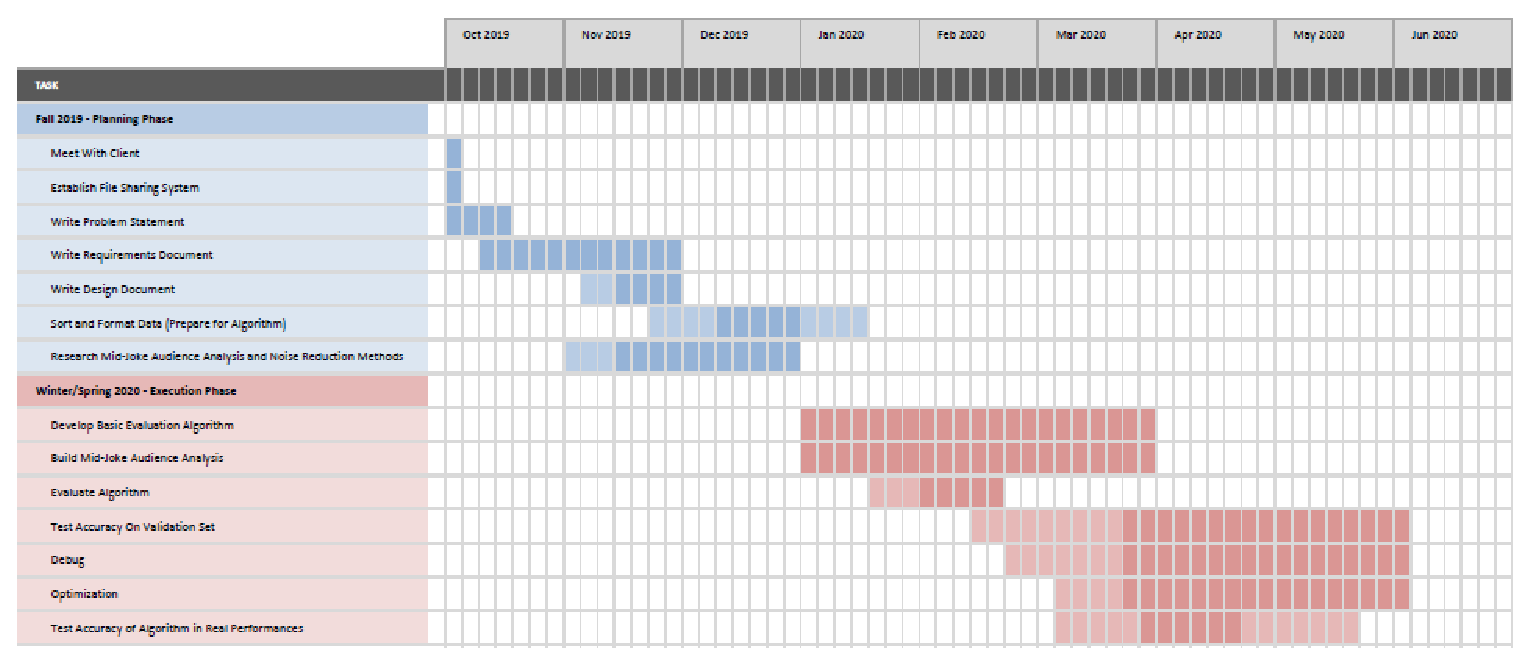
\includegraphics[width=\linewidth]{gantt.eps}
\caption{Estimated Project Timeline}
\end{figure}

\section{Conclusion}
Our project will deliver a fully functioning system for determining the successfulness of stand-up comedy jokes told by a robot to an audience. The jokes will be categorized with one of three labels: a hit, a bomb, or a neutral response. Two separate classifiers will be created: one that analyzes the audience response mid-joke and one that analyzes the audience response post-joke. The most positive response between the two will be the final result. The final product will improve the robot comedian's success in establishing positive interpersonal communications with its audience. Outside of a comedy setting the work could have further implications in the usability of AI assistants and their ability to interpret user commands.

\end{document}